\documentclass[10pt,xcolor=dvipsnames]{beamer}
\usepackage[french]{babel}
\usepackage[utf8]{inputenc}
\usepackage[T1]{fontenc}
\usepackage{caption}
\usepackage{MnSymbol,wasysym}
\usepackage{amsmath}
\usepackage{cancel}
\usepackage[draft]{pdfcomment}
\newcommand{\pdfnote}[1]{\marginnote{\pdfcomment[icon=note]{#1}}}
\usepackage{appendixnumberbeamer}
\usepackage{comment}

\renewcommand{\thefootnote}{\fnsymbol{footnote}}



\newcommand*\Let[2]{\State #1 $\gets$ #2}
\usepackage{algorithm}
\usepackage[noend]{algpseudocode}
\usepackage{tcolorbox}

\newtcolorbox{mybox}[3][]
{
  colframe = #2!25,
  colback  = #2!10,
  coltitle = #2!20!black,  
  title    = {#3},
  #1,
}

\usetheme[progressbar=frametitle,numbering=fraction]{metropolis}
%LS:
\setbeamercolor{background canvas}{bg=white}  
\usepackage{appendixnumberbeamer}

\usepackage{booktabs}
\usepackage[scale=2]{ccicons}
\usepackage{tikz}
\usetikzlibrary{calc}
\usepackage{color}
\usepackage{mathtools}

\usetikzlibrary{shapes,snakes}
%% Color Definition
\definecolor{darkspringgreen}{rgb}{0.09, 0.45, 0.27}


\setbeamertemplate{frame footer}{Rohan Fossé}

\setbeamercolor{footline}{fg=gray}

\def\checkmark{\tikz\fill[scale=0.4,color=darkspringgreen](0,.35) -- (.25,0) -- (1,.7) -- (.25,.15) -- cycle;}
\usepackage{pgfplots}
\usepgfplotslibrary{dateplot}

\usepackage{eso-pic}
\usepackage{xspace}
\long\def\/*#1*/{}

\title{
Algorithmique et structure de données
}
\subtitle{Récursivité et tableaux}

\date{\centering 30 Septembre 2021}
\author{\centering \bf Rohan Fossé}


\begin{document}

\maketitle


\section{Avant de commencer}

\begin{frame}{Supports de cours}
    \begin{alertblock}{Supports de cours}
    \begin{itemize}
        \item Site Web: \underline{labri.fr/perso/rfosse}
        \item Enoncé et Correction des EI
        \item Exercices supplémentaires
    \end{itemize}
    \end{alertblock}
\end{frame}

\begin{frame}{Rappel de la dernière séance}
    \begin{alertblock}{Complexité d'un algorithme}
    \begin{itemize}
        \item La complexité permet d'évaluer l'efficacité d'un algorithme;
        \item Elle permet de comparer des algorithmes indépendamment des machines;
        \item On note $\mathcal{O}$ la complexité asymptotique (\textit{dans le pire cas}).
    \end{itemize}
    \end{alertblock}
\end{frame}

\section{Algorithmes Récursifs}


\begin{frame}{Introduction}
    \begin{itemize}
        \item Les \alert{\textbf{algorithmes récursifs}} et les \alert{\textbf{fonctions récursives}} sont fondamentaux en informatique. Un algorithme est dit récursif s'il s'appelle \textbf{lui-même};
        \item Les premiers langages de programmation qui ont introduit la récursivité sont \texttt{LISP} et \texttt{Algol 60} et maintenant tous les langages de programmation modernes proposent une implémentation de la récursivité;
        \item On oppose généralement les algorithmes récursifs aux algorithmes dits \alert{impératifs} ou \alert{itératifs} qui s'exécutent sans invoquer ou appeler explicitement l'algorithme lui-même.
    \end{itemize}
\end{frame}



\begin{frame}{Lien avec les mathématiques : la factorielle}
On souhaite calculer $n!$. On rappelle que pour tout entier $n \geq 0$

\begin{equation*}
    n! = \prod_{i=1}^{n} i = 1 \times 2 \times \ldots \times n
\end{equation*}

\uncover<2->{On peut déduire de cette définition la propriété importante suivante

\begin{equation*}
    \forall n \geq 1, n! = n \times (n - 1)!
\end{equation*}

et donc si on sait calculer (n-1)! alors on sait calculer n!.
}

\uncover<3->{
Par ailleurs, on sait que 0! = 1. On sait donc calculer 1!, puis 2!, et par récurrence on peut établier qu'on sait calculer n! pour tout entier $n \geq 0$.
}
\end{frame}



\begin{frame}{Algorithme de la factorielle}
L'algorithme récursif de calcul de la factorielle distingue deux cas. Le premier cas ne nécessite aucun calcul, le second utilise la fonction $fact$ pour calculer $(n-1)!$

\begin{tcolorbox}
  \begin{algorithmic}[1]
    \Function{fact}{$n$}
      \If{ n == 0 }
        \State\text{\textbf{return}} 1
      \Else
        \State\text{\textbf{return}} $n \times fact(n-1)$
      \EndIf
    \EndFunction
  \end{algorithmic}
\end{tcolorbox}

\end{frame}

\begin{frame}{Exécution de l'algorithme de la factorielle}

Prenons l'exemple du déroulement du calcul récursif de $4!$ :
\begin{center}
    \begin{itemize}[<+->]
\item[] $fact(4) \rightarrow 4 \times fact(3)$
\item[] $fact(4) \rightarrow 4 \times 3 \times fact(2)$
\item[] $fact(4) \rightarrow 4 \times 3 \times 2 \times fact(1)$
\item[] $fact(4) \rightarrow 4 \times 3 \times 2 \times 1 \times fact(0)$
\item[] $fact(4) \rightarrow 4 \times 3 \times 2 \times 1 \times 1$
\item[] $fact(4) \rightarrow 24$
\end{itemize}
\end{center}
\end{frame}

\begin{frame}{Autre algorithme de factorielle}
    Considérons l'algorithme suivant :
    
    \begin{tcolorbox}
  \begin{algorithmic}[1]
    \Function{$fact2$}{$n$}
        \State\text{\textbf{return}} $n \times fact(n-1)$
    \EndFunction
  \end{algorithmic}
\end{tcolorbox}

\uncover<2->{\alert{Quel est le soucis avec cette fonction ?}}

\uncover<3->{L'évaluation de $fact2(1)$ conduit à un calcul infini:}
\end{frame}

\begin{frame}{Exécution de l'algorithme de la factorielle}

Prenons l'exemple du déroulement du calcul récursif de $4!$:
\begin{center}
    \begin{itemize}[<+->]
\item[] $fact2(1) \rightarrow 1 \times fact2(0)$
\item[] $fact2(1) \rightarrow 1 \times 0 \times fact2(-1)$
\item[] $fact2(1) \rightarrow 1 \times 0 \times -1 \times fact2(-2)$
\item[] $fact2(1) \rightarrow \ldots $
\end{itemize}
\end{center}

\end{frame}


\begin{frame}{Règle implicite de conception d'un algorithme récursif}
    \begin{exampleblock}{Règle implicite}
        Tout algorithme récursif doit distinguer plusieurs cas dont l'un au moins ne doit pas contenir d'appels récursifs.
    \end{exampleblock}
    
    Les cas non récursifs d'un algorithme récursif sont appelés \alert{\textit{cas de bases}}. Les conditions que doivent satisfaire les données dans ces cas de bases sont appelées \alert{\textit{conditions de terminaison}}.
    
    \uncover<2>{\begin{center}
        \alert{Est-ce-que c'est suffisant ?}
    \end{center}  }
\end{frame}

\begin{frame}{Reprenons notre exemple de la factorielle}
    
    \begin{tcolorbox}
  \begin{algorithmic}[1]
    \Function{fact3}{$n$}
      \If{ n == 0 }
        \State\text{\textbf{return}} 1
      \Else
        \State\text{\textbf{return}} $n \times fact3(n+1)$
      \EndIf
    \EndFunction
  \end{algorithmic}
\end{tcolorbox}
    \uncover<2->{\alert{Quel est le soucis avec cette fonction ?}}

    \uncover<3->{L'évaluation de $fact3(1)$ conduit à un calcul infini:
}
\end{frame}

\begin{frame}{Exécution de l'algorithme de la factorielle}

Prenons l'exemple du déroulement du calcul récursif de $4!$:
\begin{center}
    \begin{itemize}[<+->]
\item[] $fact3(1) \rightarrow 1 \times fact3(2)$
\item[] $fact3{1} \rightarrow 1 \times 2 \times fact3(3)$
\item[] $fact3{1} \rightarrow 1 \times 2 \times 3 \times \ldots$
\end{itemize}
\end{center}

\end{frame}

\begin{frame}{Deuxième règle implicite}
        \begin{tcolorbox}
  \begin{algorithmic}[1]
    \Function{fact3}{$n$}
      \If{ n == 0 }
        \State\text{\textbf{return}} 1
      \Else
        \State\text{\textbf{return}} $n \times fact3(n+1)$
      \EndIf
    \EndFunction
  \end{algorithmic}
\end{tcolorbox}
\uncover<2>{
\begin{exampleblock}{Deuxième règle}
À chaque appel récursif il faut se rapprocher des conditions de terminaison.
\end{exampleblock}
}
\end{frame}



\begin{frame}{Un autre exemple: les tours de Hanoï}
    \begin{alertblock}{Principe du jeu}
    \begin{itemize}
        \item On dispose de 3 tours côte à côte sur lesquelles on peut empiler des disques de diamètre croissant;
        \item On ne peut déplacer qu'un disque à la fois et on ne doit pas poser un disque plus large sur un plus petit;
        \item L'objectif est de trouver la suite de déplacements qui permet de placer tous les disques sur la tour la plus à droite.
    \end{itemize}
    \end{alertblock}
    
    \begin{figure}
        \centering
        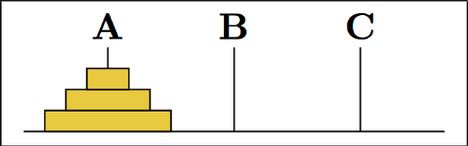
\includegraphics[scale=0.4]{figures/CM1/Hanoi-initial.png}
        \label{fig:my_label}
    \end{figure}
    \uncover<2>{\centering \alert{À vous de jouer ! En combien de mouvements est-ce possible ?}}
\end{frame}

\begin{frame}{Résolution du problème de Hanoï}
    \only<1->{\centering \alert{\textbf{La réponse: 7 !}}}
    \only<2->{\begin{figure}
        \centering
        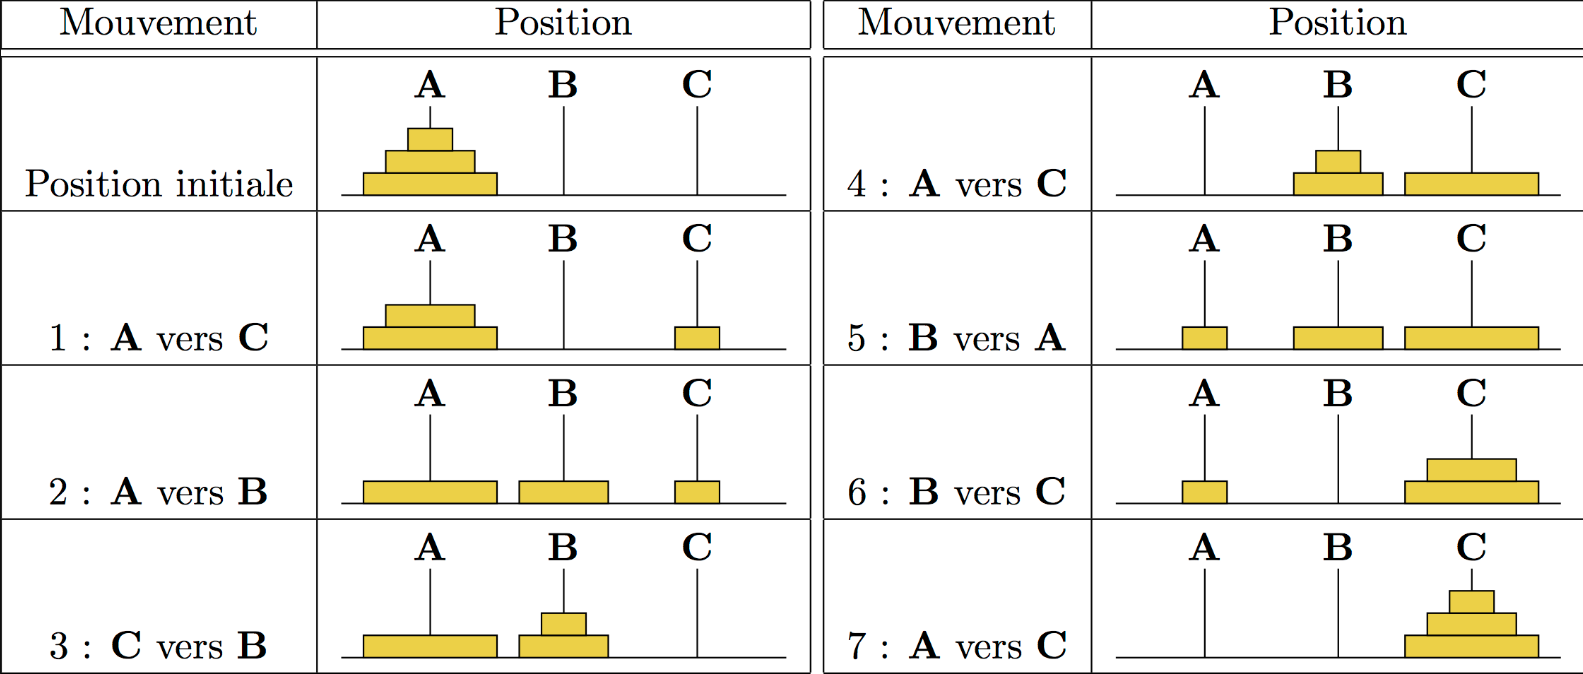
\includegraphics[scale=0.18]{figures/CM1/Hanoi.png}

        \label{fig:my_label2}
    \end{figure}
    }
\uncover<3>{\centering \alert{Quel est l'algorithme ?}}
\end{frame}

\begin{frame}{Algorithme de résolution des tours de Hanoï dans le cas général}
    Cet algorithme est la fonction $hanoi$ qui prend trois paramètres:
    \begin{enumerate}
        \item \alert{n} le nombre de disques à déplacer;
        \item \alert{d} la tour de départ où se trouvent ces disques;
        \item \alert{a} la tour d'arrivée où doivent aller les disques
    \end{enumerate}
    On suppose que l'on a une fonction $deplacerdisque(d,a)$ qui permet de déplacer un disque de $d$ jusqu'à $a$.
    \uncover<2>{  
        \begin{tcolorbox}

  \begin{algorithmic}[1]
    \Function{hanoi}{$n,d,a$}
      \If{ $n > 0 $}
        \Let{$aux$}{$\text{le piquet différent de d et a}$}
        \State $hanoi(n - 1, d, aux)$
        \State $deplacerdisque(d,a)$
        \State $hanoi(n - 1, aux, a)  $
      \EndIf
    \EndFunction
  \end{algorithmic}
\end{tcolorbox}
}
\end{frame}

\begin{frame}{Petit exercice}
    \begin{alertblock}{Exercice}
    Écrire une fonction qui calcule la somme des inverses des carrés des $n$ premiers entiers naturels non nuls.
    \end{alertblock}
    \uncover<2>{
    
    \begin{tcolorbox}

  \begin{algorithmic}[1]
    \Function{$sum\_inv$}{$n$}
      \If{ $n == 0 $}
          \State \textbf{return} 1
      \Else
          \State \textbf{return} $1/n**2 + sum\_inv(n-1)$
      \EndIf
    \EndFunction
  \end{algorithmic}
\end{tcolorbox}
    }
\end{frame}

\section{Type de récursivité}

\begin{frame}{Récursivité simple ou linéaire}
    Un algorithme récursif est \textit{simple} ou \textit{linéaire} si chaque cas qu'il distingue se résout en au plus un appel récursif.
    
\begin{tcolorbox}

  \begin{algorithmic}[1]
    \Function{mystere}{$n$}
      \If{ $n == 0 $}
         \State\text{\textbf{return}} 1
       \Else
       \State\text{\textbf{return}} $mystere(n - 1) \times 2$
      \EndIf
    \EndFunction
  \end{algorithmic}
  
\end{tcolorbox}

\uncover<2>{\centering \alert{Que fait cet algorithme ?}}
    
\end{frame}


\begin{frame}{Récursivité terminale}
\uncover<1-4>{Une définition de fonction f est récursive terminale quand tout appel récursif est de la forme return f(...); La valeur retournée est directement la valeur obtenue par un appel récursif, sans qu'il n'y ait aucune opération sur cette valeur.
}
 \vspace{-0.05cm}
\uncover<2->{
\begin{tcolorbox}

  \begin{algorithmic}[1]
    \Function{$recursionTerminale$}{$n$}
         \State\text{\textbf{...}} 
       \State\text{\textbf{return}} $recursionTerminale(n - 1)$
    \EndFunction
  \end{algorithmic}
 \end{tcolorbox}
 
 }
 
 \vspace{-0.05cm}
 
 \uncover<3->{
 \begin{tcolorbox}
    \begin{algorithmic}[1]
    \Function{$recursionNonTerminale$}{$n$}
         \State\text{\textbf{...}} 
       \State\text{\textbf{return}} $n + recursionTerminale(n - 1)$
    \EndFunction
  \end{algorithmic}
  
\end{tcolorbox}
}
 \vspace{-0.2cm}
\uncover<4->{
Dans le premier cas, aucune référence aux résultats précédents n'est à conserver en mémoire, tandis que dans le second cas, tous les résultats intermédiaires doivent l'être.
}
\end{frame}

\begin{frame}{Et la fonction factorielle ?}
    Reprenons la fonction $factorielle$
    \begin{tcolorbox}
  \begin{algorithmic}[1]
    \Function{fact}{$n$}
      \If{ n == 0 }
        \State\text{\textbf{return}} 1
      \Else
        \State\text{\textbf{return}} $n \times fact(n-1)$
      \EndIf
    \EndFunction
  \end{algorithmic}
\end{tcolorbox}
    \uncover<2->{\centering \alert{Est-elle récursive terminale ?}}
    \uncover<3>{\centering \alert{Non, il y a une multiplication par n avant de retourner.}}
\end{frame}

\begin{frame}{Exemple d'une fonction récursive terminale}
        \begin{tcolorbox}
  \begin{algorithmic}[1]
    \Function{f}{$n,a$}
      \If{ n <= 1 }
        \State\text{\textbf{return}} a
      \Else
        \State\text{\textbf{return}} $f(n-1,n*a)$
      \EndIf
    \EndFunction
  \end{algorithmic}
\end{tcolorbox}
     \uncover<2->{\centering \alert{Que fait cette fonction ?}}
\end{frame}

\begin{frame}{Avantage de la récursivité terminale}
    \begin{itemize}
        \item     La plupart des langages fonctionnels (comme \textit{LISP} et \textit{CAML}) exécutent un programme à récursivité terminale comme s'il était itératif, c'est-à-dire en espace constant.
        \item Une fonction récursive terminale peut toujours être transformée en itération.
    \end{itemize}


\end{frame}

\begin{frame}{Petit exercice}
    \begin{alertblock}{Transformer cette fonction récursive terminale en itération}
                \begin{tcolorbox}
  \begin{algorithmic}[1]
    \Function{f}{$n,a$}
      \If{ n <= 1 }
        \State\text{\textbf{return}} a
      \Else
        \State\text{\textbf{return}} $f(n-1,n*a)$
      \EndIf
    \EndFunction
  \end{algorithmic}
\end{tcolorbox}
    \end{alertblock}
    
    \uncover<2>{
    \begin{tcolorbox}
  \begin{algorithmic}[1]
    \Function{f}{$n$}
      \Let{$a$}{$1$}
      \While{ n > 1 }
        \Let{$a$}{$n*a$}
        \Let{$n$}{$n-1$}
      \EndWhile
        \State\text{\textbf{return}} $a$

    \EndFunction
  \end{algorithmic}
\end{tcolorbox}
    
    }
\end{frame}

\begin{frame}{Récursivité multiple}
\begin{exampleblock}{Définition}
        Un algorithme récursif est multiple si l’un des cas qu’il distingue se résout avec plusieurs appels récursifs.
\end{exampleblock}
Prenons la suite de fibonacci comme exemple

\begin{equation}
                fibo(n)=\begin{cases} 1 &, \text{si $n=0$}.\\ 1 &, \text{si $n=1$}.\\ fibo(n-1) + fibo(n-2) &, \text{si $n>1$}. \end{cases} 
\end{equation}
\end{frame}



\begin{frame}{Récursivité croisée}
    \begin{exampleblock}{Définition}
Deux algorithmes sont dits mutuellement récursifs si l’un fait appel à l’autre et l’autre à l’un. On parle aussi de récursivité croisée.
\end{exampleblock}

\begin{tcolorbox}
  \begin{algorithmic}[1]
    \Function{pair}{$n$}
        \If{$n == 0$}
        \State \textbf{return} True
        \Else
        \State \textbf{return} $impair(n - 1)$
        \EndIf
    \EndFunction
  \end{algorithmic}
  
    \begin{algorithmic}[1]
    \Function{impair}{$n$}
        \If{$n == 0$}
        \State \textbf{return} False
        \Else
        \State \textbf{return} $pair(n - 1)$
        \EndIf
    \EndFunction
  \end{algorithmic}
\end{tcolorbox}

\end{frame}


\section{Recherche dans un tableau}

\begin{frame}{Algorithme de recherche d'un élément dans un tableau}
    \begin{tcolorbox}
  \begin{algorithmic}[1]
    \Function{search}{$tab,e$}
        \For{$i < tab.size$}
        
        \If{$tab[i] == e$}
            \State \textbf{return} $i$
        \EndIf
    \EndFor
    \State \textbf{return} nonTrouvé
    \EndFunction
  \end{algorithmic}
\end{tcolorbox}

\uncover<2->{\centering \alert{Quelle est la complexité de cette fonction ?}} 
\uncover<3>{$\mathcal{O}(n)$}

\end{frame}

\begin{frame}{Recherche d'un élément dans un tableau}
    La complexité précédente est trop élevée, surtout sachant que la recherche dans un tableau est une opération de base utilisée dans de nombreux algorithmes.\\
    
    Pour aller plus vite, on peut utiliser les \textbf{tableaux triés} et la \textbf{dichotomie}.
\end{frame}

  
\begin{frame}{Exemple : La dichotomie}
    \begin{exampleblock}{Definition}
    La recherche dichotomique, ou recherche par dichotomie (en anglais : \textit{binary search}), est un algorithme de recherche pour trouver la position d'un élément dans un tableau trié.
    \end{exampleblock}
\begin{alertblock}{Le principe}
L'objectif est trouver la position d'un élément dans un tableau trié.
\begin{itemize}
    \item On trouve l'élément $m$ avec la position la plus centrale du tableau (si le tableau est vide on s'arrête);
    \item On compare la valeur de l'élément recherché avec l'élément $m$;
    \item Si elle est plus petite, on recommence dans le sous-tableau de gauche, sinon dans le sous-tableau de droite.
\end{itemize}
\end{alertblock}

\end{frame}

\begin{frame}{L'algorithme de la dichotomie}
    
\begin{tcolorbox}
  \begin{algorithmic}[1]
    \Function{dichotomie}{$tab,min,max,e$}
        
        \If{$min == max$}
            \If{$tab[min] = e$}
                \State \textbf{return} $min$
        \Else
            \State \textbf{return} nonTrouvé
            \EndIf
        \EndIf
    \Let{$mid$}{$( min + max ) / 2$}
    \If{$tab[mid] < e$}
        \State \textbf{return} $dichotomie(tab, mid+1, max, e)$
    \Else
        \State \textbf{return} $dichotomie(tab, min, mid, e)$
    \EndIf
    \EndFunction
  \end{algorithmic}
\end{tcolorbox}

\uncover<2->{\centering \alert{Quelle est la complexité de cette fonction ?}} 
\uncover<3>{$\mathcal{O}(log_2(n))$}

\end{frame}

\begin{frame}{L'algorithme de la dichotomie itérative}
    
\begin{tcolorbox}
  \begin{algorithmic}[1]
    \Function{dichotomie}{$tab,e$}
    \Let{$min$}{$0$}
    \Let{$max$}{$\text{taille - 1}$}
    \While{$min < max$}
        \Let{$mid$}{$( min + max ) / 2 $}
        \If{$tab[mid] < e$}
            \Let{$min$}{$mid+1$}
        \Else
            \Let{$max$}{$mid$}
        \EndIf
    \EndWhile 
    \If{$\text{tab[min] == e}$}
        \State \textbf{return} $min$
    \Else
        \State \textbf{return} nonTrouvé
    \EndIf
    \EndFunction
  \end{algorithmic}
\end{tcolorbox}

\vspace{-0.2cm}

\uncover<2->{\centering \alert{Quelle est la complexité de cette fonction ?}} 
\uncover<3>{$\mathcal{O}(log_2(n))$}

\end{frame}

\begin{frame}{Exercice}
    \begin{exampleblock}{Exercice}
        Déterminer la version itérative de l'algorithme de la dichotomie
    \end{exampleblock}
\end{frame}

\begin{frame}{L'algorithme de la dichotomie itérative (variante)}

\begin{tcolorbox}
  \begin{algorithmic}[1]
    \Function{dichotomie}{$tab,e$}
    \Let{$min$}{$0$}
    \Let{$max$}{$\text{taille - 1}$}
    \While{$min < max$}
        \Let{$mid$}{$( min + max ) / 2 $}
        \If{$tab[mid] == e$}
            \State \textbf{return} $mid$
        \EndIf
        \If{$tab[mid] < e$}
            \Let{$min$}{$mid+1$}
        \Else
            \Let{$max$}{$mid$}
        \EndIf
    \EndWhile 
    \If{$tab[min] == e$}
        \State \textbf{return} $min$
    \Else
        \State \textbf{return} nonTrouvé
    \EndIf
    \EndFunction
  \end{algorithmic}
\end{tcolorbox}

\uncover<2->{\centering \alert{Quelle est la complexité de cette fonction ?}} 
\uncover<3>{$\mathcal{O}(log_2(n))$}


\end{frame}

\begin{frame}{Autres applications de la recherche dichotomique}

\begin{itemize}
    \item Jeu du nombre inconnu où l'on répond soit "plus grand" soit "plus petit" soit "gagné";
    \item Calcul d'une racine d'une fonction croissante;
    \item Algorithme de pointage et de visée;
    \item Recherche de l'apparition d'un bug dans l'histoire d'un programme.
\end{itemize}
\end{frame}

\section{Tri de tableaux et algorithmes de tris}

\begin{frame}{Insertion dans un tableau trié}
    \begin{tcolorbox}
  \begin{algorithmic}[1]
    \Function{Insertion}{$tab,e$}
    \Let{$i$}{$taille$}

    \While{$\text{i > 0 and tab[i - 1] > e}$}
        \Let{$tab[i]$}{$tab[i - 1]$}
        \Let{$i$}{$i - 1$}
    \EndWhile
    \Let{$tab[i]$}{$e$}
    \Let{$taille$}{$taille + 1$}
    \EndFunction
  \end{algorithmic}
\end{tcolorbox}

\uncover<2->{\centering \alert{Quelle est la complexité de cette fonction ?}} 
\uncover<3>{$\mathcal{O}(n)$}

\end{frame}

\begin{frame}{Tri par insertion}
    \begin{tcolorbox}
  \begin{algorithmic}[1]
    \Function{Insertsort}{$tab$}
    \Let{$i$}{$1$}
    \For{$i < taille$}
        \Let{$e$}{$t[i]$}
        \Let{$j$}{$i$}
        \While{$\text{j > 0 and tab[j - 1] > e}$}
            \Let{$tab[j]$}{$tab[j - 1]$}
            \Let{$j$}{$j - 1$}
        \EndWhile
        \Let{$tab[j]$}{$e$}
    \EndFor
    \EndFunction
  \end{algorithmic}
\end{tcolorbox}

\uncover<2->{\centering \alert{Quelle est la complexité de cette fonction ?}}
\uncover<3>{$\mathcal{O}((n^2))$}

\end{frame}



\section{Diviser pour régner}
\begin{frame}{Approche diviser pour régner}
En informatique, \textbf{\alert{diviser pour régner}} est une technique algorithmique consistant à : 
  \begin{enumerate}
  \item \alert{Diviser} : découper un problème initial en sous-problèmes;
  \item \alert{Régner} : résoudre les sous-problèmes (récursivement ou directement s'ils sont assez petits);
  \item \alert{Combiner} : calculer une solution au problème initial à partir des solution des sous-problèmes.
  \end{enumerate}
  
 \uncover<2>{\alert{\textbf{Comment obtenir un tableau trié, si l'on sait trier chaque moitié ?}}}

  \end{frame}
 
 
 \begin{frame}{Fusion de tableaux triés}
            \begin{tcolorbox}
  \begin{algorithmic}[1]
    \Function{$fusion$}{$A[a_1,a_2,\ldots,a_n],B[b_1,b_2,\ldots,b_n]$}
        \If{$\text{A est vide}$}
            \State \textbf{return} B
        \EndIf
        \If{$\text{B est vide}$}
            \State \textbf{return} A
        \EndIf
        \If{$A[a_1] <= B[b_1]$}
            \State \textbf{return} A[$a_1$] + fusion($A[a_2,\ldots,a_n],B$)
        \Else
            \State \textbf{return} B[$b_1$] + fusion($A, B[b_2,\ldots,b_n]$)   
        \EndIf
    \EndFunction
  \end{algorithmic}
\end{tcolorbox}


     \uncover<2->{\centering \alert{Quelle est la complexité de cette fonction ?}} 
     \uncover<3>{$\mathcal{O}((t_a + t_b))$}
     
 \end{frame}

\begin{frame}{Tri par fusion (MergeSort)}
                \begin{tcolorbox}
  \begin{algorithmic}[1]
    \Function{$trifusion$}{$T[t_1,t_2,\ldots,t_n]$}
        \If{$t_n <= 1$}
            \State \textbf{return} T
        \Else
            \State \textbf{return} fusion(triFusion(T[$t_1, \ldots, t_{n/2}$]), triFusion(T[$t_{n/2 + 1}, \ldots, t_n$]))
        \EndIf
    \EndFunction
  \end{algorithmic}
\end{tcolorbox}

     \uncover<2->{\centering \alert{Quelle est la complexité de cette fonction ?}} 
     \uncover<3>{$\mathcal{O}((t_a + t_b))$}
\end{frame}


\section{Complexité d'un algorithme diviser pour régner}

\begin{frame}{La complexité}
Le temps d'exécution d'un algorithme \textit{diviser pour régner} se décompose suivant les trois étapes du paradigme de base.


\begin{itemize}
    \item \alert{Diviser}: le problème en $\textbf{\alert{a}}$ sous-problèmes chacun de taille $\textbf{\alert{n/b}}$. Soit $\textbf{\alert{D(n)}}$ le temps nécessaire à la division du problème en sous-problèmes;
    \item \alert{Régner}: soit $\textbf{\alert{a T(n/b)}}$ le temps de résolution des $\textbf{\alert{a}}$ sous-problèmes;
    \item \alert{Combiner}: soit $\textbf{\alert{C(n)}}$ le temps nécessaire pour construire la solution finale à partir des solutions aux sous-problèmes.
\end{itemize}
    
Finalement, le temps d'exécution global de l'algorithme est:
\begin{equation*}
    T(n) = a T(n/b) + D(n) + C(n)
\end{equation*}

Soit la fonction $f(n)$ qui regroupe D(n) et C(n). T(n) est alors définie de la façon suivante:
\begin{equation*}
    T(n) = a T(n/b) + f(n)
\end{equation*}
\uncover<2->{\centering \alert{On s'appelle ce théorème le \textit{master theorem}}}
\end{frame}

\begin{frame}{Théorème de résolution de la récurrence}
\begin{exampleblock}{Master theorem}
\begin{equation*}
    T(n) = a T(n/b) + f(n)
\end{equation*}
\end{exampleblock}


Supposons que $f(n) = c*n^k$, on a : $T(n) = a T(n/b) + c n^k$

\begin{equation*}
    a > b^k \rightarrow T(n) = \mathcal{O}(n^{log_b a})
\end{equation*}
\begin{equation*}
    a = b^k \rightarrow T(n) = \mathcal{O}(n^k log_b n)
\end{equation*}
\begin{equation*}
    a < b^k \rightarrow T(n) = \mathcal{O}( f(n) ) = O(n^k)
\end{equation*}
\end{frame}



\begin{frame}{Recherche Dichotomique : Arbre récursif}
  \begin{minipage}{.3\linewidth}
    \begin{tikzpicture}[invis/.style={draw=none}]
    \tikzstyle{level 1}=[edge from parent/.style={draw}, sibling distance=17mm]
    \tikzstyle{level 3}=[edge from parent/.style={draw,dashed}, sibling distance=17mm]
    \tikzstyle{level 5}=[edge from parent/.style={draw=none}, sibling distance=17mm]
    \tikzstyle{level 10}=[edge from parent/.style={draw=none}, level distance=5mm]
    \tikzstyle{level 11}=[edge from parent/.style={draw=none}, level distance=15mm]
    \tikzstyle{every node}=[fill=white,rectangle, rounded corners,draw=black,solid,minimum width=14mm]
    \tikzstyle{every node}=[fill=white,rectangle, rounded corners,draw=black,solid,minimum width=14mm]
    \node {$n$}
    child {node {$n/2$}
      child {node {$n/4$}
        child {node {$n/2^k$}
          child {node {$1$}
            child[grow=right] {node[invis] {$\log_2 n$}
              child[grow=up] {node[invis] {$k$}
                child[grow=up] {node[invis] {2}
                  child[grow=up] {node[invis] {1}
                    child[grow=up] {node[invis] {0}
                      child[grow=up] {node[invis] {niveaux}
                        child[grow=left] {node[invis] {taille}
                        }
                      }
                  }
                }
              }
            }
          }
        }
      }
    }
};
  \end{tikzpicture}
\end{minipage}
\hfill\begin{minipage}[r]{.6\linewidth}
  \only<2->{Niveau $k$}
  \begin{itemize}
  \item<2-> $\mathbf{1}$ sous problème de taille $\mathbf{n/2^k}$
  \item<2-> $\mathcal{O}(1)$ opérations élémentaires  par niveau
  \end{itemize}
  \uncover<3->{Total:}
  \begin{itemize}
  \item<3-> taille du problème divisée par 2 à chaque niveau $\implies \log_2 n +1$ niveaux.
  \item<4-> \underline{Complexité} = $\mathcal{O}(\log n)$
\end{itemize}
\end{minipage}
\end{frame}

\begin{frame}{En utilisant le \textit{master theorem}}
\begin{minipage}{.39\linewidth}
  \begin{itemize}
    \item \alert{Diviser}: le problème en $\textbf{\alert{a}}$ sous-problèmes chacun de taille $\textbf{\alert{n/b}}$. Soit $\textbf{\alert{D(n)}}$ le temps nécessaire à la division du problème en sous-problèmes;
    \item \alert{Régner}: soit $\textbf{\alert{a T(n/b)}}$ le temps de résolution des $\textbf{\alert{a}}$ sous-problèmes;
    \item \alert{Combiner} : soit $\textbf{\alert{C(n)}}$ le temps nécessaire pour construire la solution finale à partir des solutions aux sous-problèmes.
\end{itemize}
\end{minipage}
\begin{minipage}{.59\linewidth}
  \begin{algorithmic}[1]
    \Function{dichotomie}{$tab,min,max,e$}
        
        \If{$min == max$}
            \If{$tab[min] = e$}
                \State \textbf{return} $min$
            \EndIf
        \Else
            \State \textbf{return} nonTrouvé
        \EndIf
    \Let{$mid$}{$( min + max ) / 2$}
    \If{$tab[mid] < e$}
        \State \textbf{return} $dichotomie(tab, mid+1, max, e)$
    \Else
        \State \textbf{return} $dichotomie(tab, min, mid, e)$
    \EndIf
    \EndFunction
  \end{algorithmic}
\end{minipage}

\end{frame}

\begin{frame}{Complexité de recherche dichotomique}
    \begin{alertblock}{Rappel}
    Supposons que $f(n) = c*n^k$, on a : $T(n) = a T(n/b) + c n^k$

\begin{equation*}
    a > b^k \rightarrow T(n) = \mathcal{O}(n^{log_b a})
\end{equation*}
\begin{equation*}
    a = b^k \rightarrow T(n) = \mathcal{O}(n^k log_b n)
\end{equation*}
\begin{equation*}
    a < b^k \rightarrow T(n) = \mathcal{O}( f(n) ) = O(n^k)
\end{equation*}
    \end{alertblock}

On a \alert{a = 1, b = 2, k = 0} $\rightarrow$ a = $b^k$

D'après le théorème, on a donc :

\begin{equation*}
    T(n) = \mathcal{O}(n^k log_b n) = \mathcal{O}(log(n))
\end{equation*}
% 
\end{frame}    
\end{document}

